\documentclass[a4paper, 12pt]{article}

% <--------- Packages ---------> %

\usepackage{fullpage}   % Package to use full page
\usepackage{tikz}       % Package for drawing
\usepackage{pdfpages}
\usepackage{fancyhdr}
\usepackage{array}
\usepackage{tabularx}
\usepackage{colortbl}
\usepackage{pgfplots}
\usepackage{xcolor}
\usepackage{float}
\usepackage[normalem]{ulem}

% <--------- Mathematics ---------> %

\usepackage{amssymb}   % Extra symbols
\usepackage{amsthm}  
\usepackage{amsmath}   % Theorem-like environments
\usepackage{thmtools}  % Theorem-like environments
\usepackage{mathtools} % Fonts and environments for mathematical formuale
\usepackage{mathrsfs}  % Script font with \mathscr{}

% <--------- Others ---------> %

\usepackage{indentfirst}
\usepackage[utf8]{inputenc}
\usepackage[english]{babel}
\usepackage[thinlines]{easytable}
\usepackage{caption}
% \usepackage[parfill]{parskip}
\usepackage{pgfplots}
\usepackage{multicol}
\usepackage{lipsum}


%===========================================%
%=            Page Style                   =%

\usepackage{times}

\pgfplotsset{compat=1.7}
\setlength{\parindent}{1.3em}
\renewcommand{\baselinestretch}{1.5}

%=                                         =%
%===========================================%


%===========================================%
%=            Code Setup                   =%

\usepackage{listings}
\usepackage{color}

\definecolor{dkgreen}{RGB}{163, 190, 140}
\definecolor{gray}{RGB}{59, 66, 82}
\definecolor{mauve}{RGB}{94, 129, 172}
\definecolor{lightgray}{RGB}{46, 52, 64}

\lstset{
  language={Python},
  aboveskip=0.6mm,
  belowskip=0.6mm,
  showstringspaces=false,
  columns=flexible,
  basicstyle={\small\ttfamily},
  numbers=left,
  numberstyle=\tiny\color{gray},
  keywordstyle=\color{mauve},
  commentstyle=\color{gray},
  stringstyle=\color{dkgreen},
  morekeywords={pop},
  breaklines=true,
  breakatwhitespace=true,
  tabsize=4
}

%=                                         =%
%===========================================%


%===========================================%
%=               Credits                   =%

\author{Name}
\title{Title}

%=                                         =%
%===========================================%

%===========================================%
%=               BEGIN                     =%

\begin{document}

\pgfplotsset{compat=1.17}
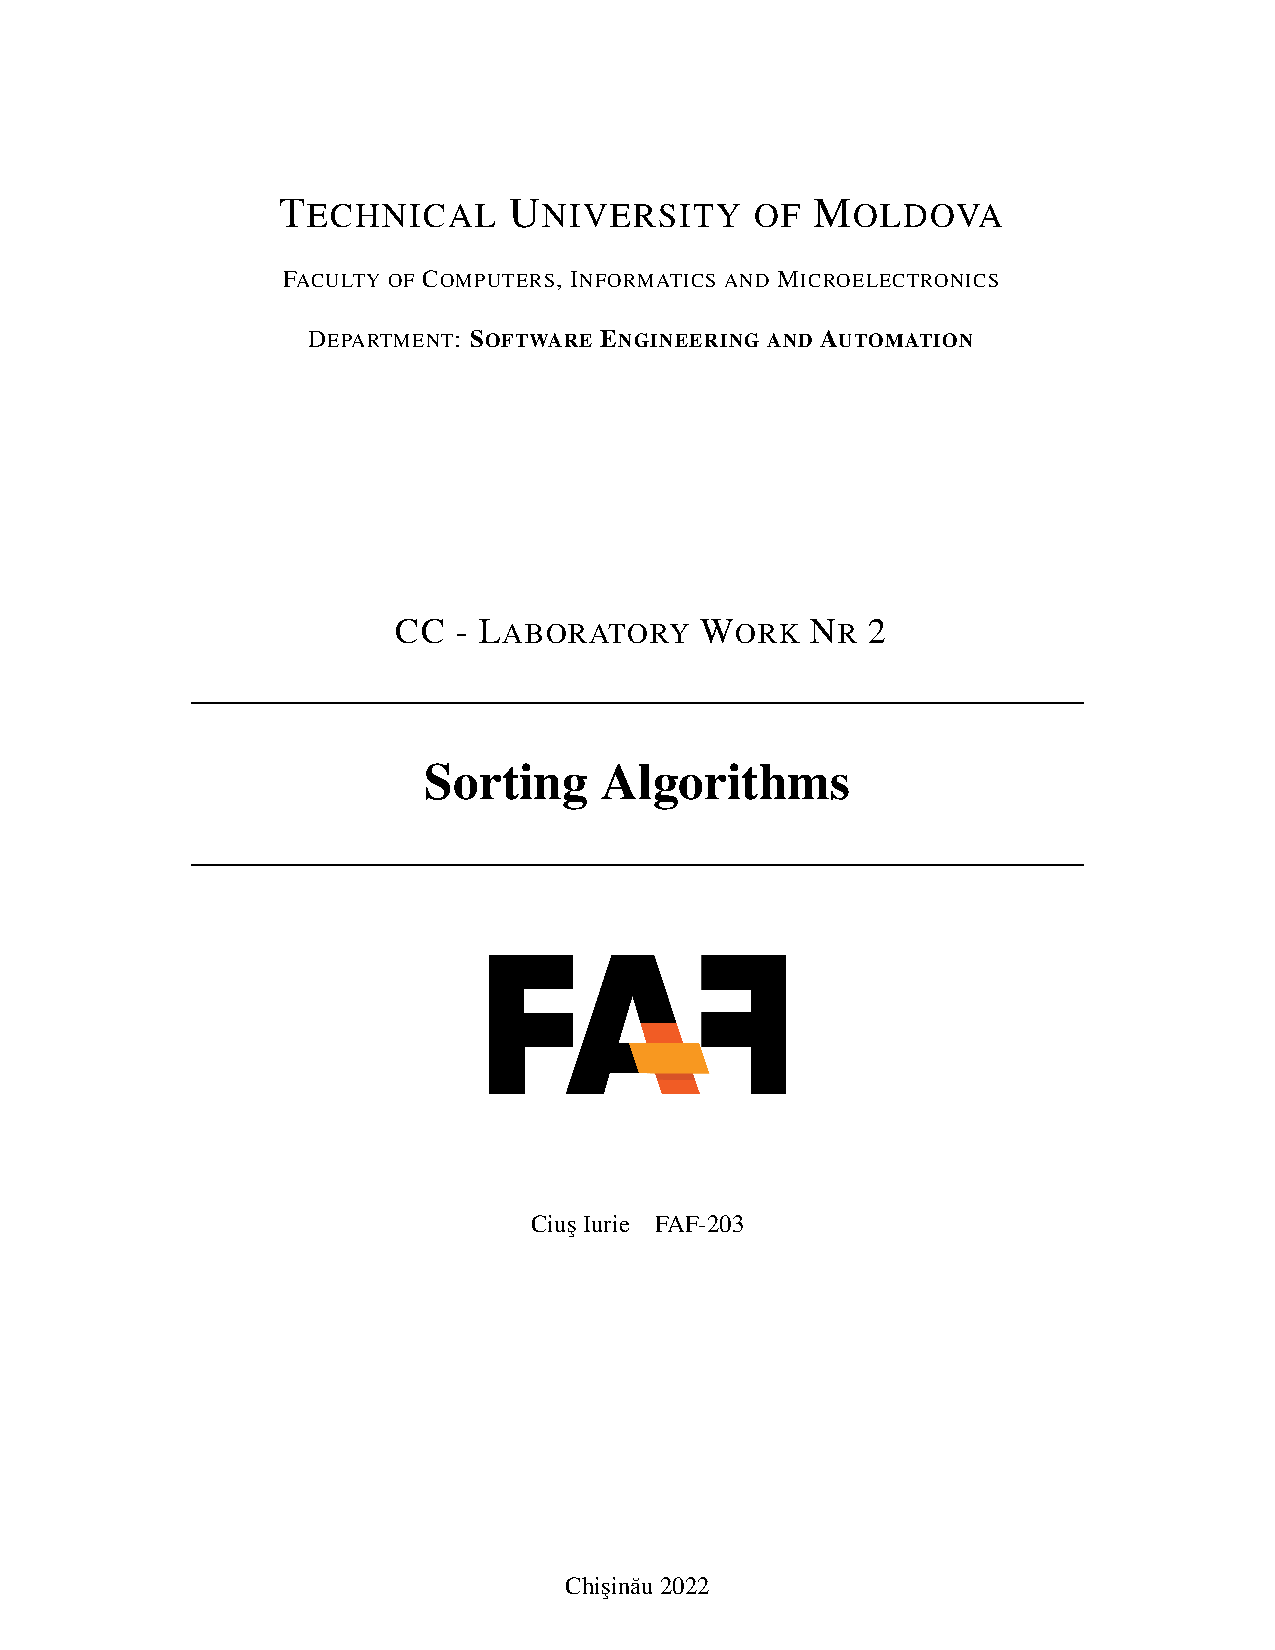
\includepdf[pages={1}]{title.pdf}
\tableofcontents

\newpage

\section{Algorithm Analysis}

Algorithm analysis is an important part of computational complexity theory, which provides
theoretical estimation for the required resources of an algorithm to solve a specific computational problem. Analysis of algorithms is the determination of the amount of time and space
resources required to execute it.

\subsection{Introduction}

The current paper work represents my implementation of five Sieve of Eratosthenes algorithms. 

\hfill \break
\indent The Sieve of Eratosthenes is a method for finding all primes up to (and possibly including) a given natural. This method works well when is relatively small, allowing us to determine whether any natural number less than or equal to is prime or composite.

It does so by iteratively marking as composite (i.e., not prime) the 
multiples of each prime, starting with the first prime number. The 
multiples of a given prime are generated as a sequence of numbers 
starting from that prime, with constant difference between them that 
is equal to that prime. This is the sieve's key distinction from 
using trial division to sequentially test each candidate number for 
divisibility by each prime. Once all the multiples of each discovered 
prime have been marked as composites, the remaining unmarked numbers are 
primes.

\subsection{Objectives}

\begin{itemize}
  \item Study and empirical analysis of sorting algorithms. QuickSort, mergeSort, heapSort analysis, (one of your choice).
  \item Establish the properties of the input data in relation to which the analysis is made.
  \item Choose the metric for comparing algorithms.
  \item Perform empirical analysis of the proposed algorithms.
  \item Make a conclusion on the work done.
\end{itemize}

\subsection{Theoretical Notes}

A prime number is a natural number that has exactly two distinct natural number divisors: the number 1 and itself.

To find all the prime numbers less than or equal to a given integer n by \textit{Eratosthenes' method}:

\begin{itemize}
  \item Create a list of consecutive integers from 2 through n: (2, 3, 4, ..., n).
  \item Initially, let p equal 2, the smallest prime number.
  \item Enumerate the multiples of p by counting in increments of p from 2p to n, and mark them in the list (these will be 2p, 3p, 4p, ...; the p itself should not be marked).
  \item Find the smallest number in the list greater than p that is not marked. If there was no such number, stop. Otherwise, let p now equal this new number (which is the next prime), and repeat from step 3.
  \item When the algorithm terminates, the numbers remaining not marked in the list are all the primes below n.
\end{itemize}

The main idea here is that every value given to p will be prime, because if it were composite it would be marked as a multiple of some other, smaller prime. Note that some of the numbers may be marked more than once (e.g., 15 will be marked both for 3 and 5).

As a refinement, it is sufficient to mark the numbers in step 3 starting from $p^2$, as all the smaller multiples of p will have already been marked at that point. This means that the algorithm is allowed to terminate in step 4 when p2 is greater than n

Another refinement is to initially list odd numbers only, \textit{(3, 5, ..., n)}, and count in increments of $2p$ from $p^2$ in step 3, thus marking only odd multiples of p. This actually appears in the original algorithm. This can be generalized with wheel factorization, forming the initial list only from numbers coprime with the first few primes and not just from odds (i.e., numbers coprime with 2), and counting in the correspondingly adjusted increments so that only such multiples of p are generated that are coprime with those small primes, in the first place.

\subsubsection*{Example}

To find all the prime numbers less than or equal to 30, proceed as follows.

First, generate a list of integers from 2 to 30:

\begin{center}
  2  3  4  5  6  7  8  9  10 11 12 13 14 15 16 17 18 19 20 21 22 23 24 25 26 27 28 29 30
\end{center}

The first number in the list is 2; cross out every 2nd number in the list after 2 by counting up from 2 in increments of 2 (these will be all the multiples of 2 in the list):

\begin{center}
  2  3  \sout{4}  5  \sout{6}  7  \sout{8}  9  \sout{10} 11 \sout{12} 13 \sout{14} 15 \sout{16} 17 \sout{18} 19 \sout{20} 21 \sout{22} 23 \sout{24} 25 \sout{26} 27 \sout{28} 29 \sout{30}
\end{center}

The next number in the list after 2 is 3; cross out every 3rd number in the list after 3 by counting up from 3 in increments of 3 (these will be all the multiples of 3 in the list):

\begin{center}
  2  3  \sout{4}  5  \sout{6}  7  \sout{8}  \sout{9}  \sout{10} 11 \sout{12} 13 \sout{14} \sout{15} \sout{16} 17 \sout{18} 19 \sout{20} \sout{21} \sout{22} 23 \sout{24} 25 \sout{26} \sout{27} \sout{28} 29 \sout{30}
\end{center}

The next number not yet crossed out in the list after 3 is 5; cross out every 5th number in the list after 5 by counting up from 5 in increments of 5 (i.e. all the multiples of 5):

\begin{center}
  2  3  \sout{4}  5  \sout{6}  7  \sout{8}  \sout{9}  \sout{10} 11 \sout{12} 13 \sout{14} \sout{15} \sout{16} 17 \sout{18} 19 \sout{20} \sout{21} \sout{22} 23 \sout{24} \sout{25} \sout{26} \sout{27} \sout{28} 29 \sout{30}
\end{center}

The next number not yet crossed out in the list after 5 is 7; the next step would be to cross out every 7th number in the list after 7, but they are all already crossed out at this point, as these numbers (14, 21, 28) are also multiples of smaller primes because 7 × 7 is greater than 30. The numbers not crossed out at this point in the list are all the prime numbers below 30:

\begin{center}
  2  3     5     7           11    13          17    19          23                29
\end{center}

\newpage

\subsection{Algorithms}

Required algorithms to implement in a programming language.

\begin{multicols}{2}

\subsubsection{Algorithm 1}

\begin{lstlisting}
  c[1] = false;
  i = 2;
  while (i <= n){
    if (c[i] == true) {
      j = 2*i;
      while (j <= n) {
        c[j] = false;
        j = j + i;
      }
    }
    i = i + 1;
  }
\end{lstlisting}

\subsubsection{Algorithm 2}

\begin{lstlisting}
  c[1] = false;
  i = 2;
  while (i <= n) {
    j=2*i;
    while (j <= n) {
      c[j] = false;
      j = j + i;
    }
    i = i + 1;
  }
\end{lstlisting}

\hfill \break

\subsubsection{Algorithm 3}

\begin{lstlisting}
  c[1] = false;
  i = 2;
  while (i <= n) {
    if (c[i] == true) {
      j = i + 1;
      while (j <= n) {
          if (j % i == 0) {
          c[j] = false;
          }
          j = j + 1;
      }
    }
    i = i + 1;
  }
\end{lstlisting}

\subsubsection{Algorithm 4}

\begin{lstlisting}
  c[1] = false;
  i = 2;
  While (i <= n) {
    j = 2;
    while (j < i) {
      if ( i % j == 0) {
        c[i] = false
      }
      j = j + 1;
    }
    i = i + 1;
  }
\end{lstlisting}
\end{multicols}

\newpage
\subsubsection{Algorithm 5}

\begin{lstlisting}
  c[1] = faux;
  i = 2;
  while (i<=n) {
    j = 2;
    while (j <= sqrt(i)) {
      if (i % j == 0) {
        c[i] = false;
      }
      j++;
    }
    i++;
  }
\end{lstlisting}

\newpage

\section{Code}

This section shows my implementation and result for the 5 given Sieve of Eratosthenes algorithms.

\subsection{Implementation}

\lstinputlisting[language=Python]{../SIEVE.py}

\newpage

\subsection{Algorithmic complexity}

The sieve of Eratosthenes is a popular way to benchmark computer 
performance. The time complexity of calculating all primes below 
n in the random access machine model is O(n log log n) operations, 
a direct consequence of the fact that the prime harmonic series 
asymptotically approaches log log n. It has an exponential time 
complexity with regard to input size, though, which makes it a 
pseudo-polynomial algorithm. The basic algorithm requires O(n) of memory.

The bit complexity of the algorithm is O(n (log n) (log log n)) 
bit operations with a memory requirement of O(n).

The normally implemented page segmented version has the same operational 
complexity of O(n log log n) as the non-segmented version but reduces the 
space requirements to the very minimal size of the segment page plus the 
memory required to store the base primes less than the square root of the 
range used to cull composites from successive page segments of size $O(\frac{\sqrt{n}}{log(n)})$.

A special (rarely, if ever, implemented) segmented version of the sieve of Eratosthenes, 
with basic optimizations, uses O(n) operations and $O(\sqrt{n}\frac{log\ log\ n}{log \ n})$ bits of memory.

\subsection{Graph / Results}

\begin{center}
  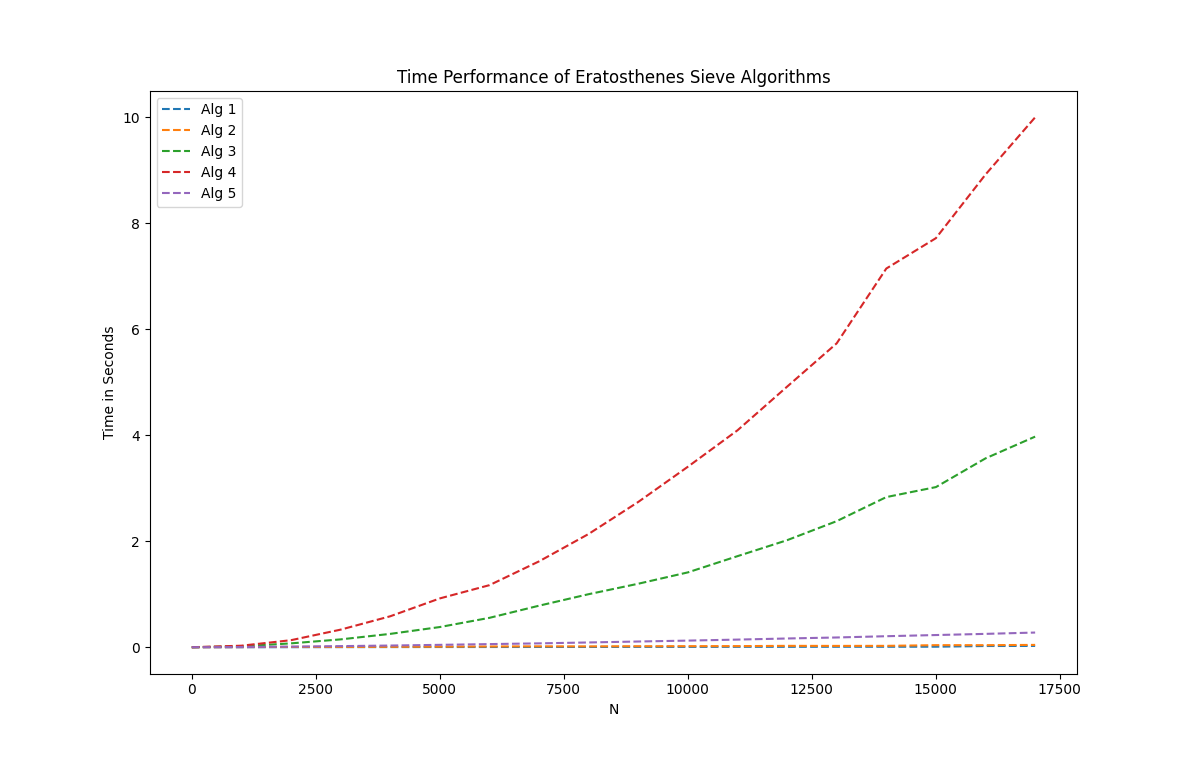
\includegraphics[width=13cm]{graph.png}
\end{center}

\newpage

\section{Conclusion}

To conclude, the current piece of work represents my personal implementation of 
5 algorithms for obtaining Eratosthenes Sieve. The programming language I chose is 
Python. The results show the time performance in seconds based on the N limit. 
As you can see in the \textit{Figure 1}, the first 3 algorithms performed the best with 
a complexity of O(0), while the last 2 - $O(n^2)$ and $O(log \ n)$.  

\subsection*{References}

\begin{itemize}
  \item https://github.com/IuraCPersonal/FAF203-CC
\end{itemize}

\end{document}

%=                END                      =%
%===========================================%